%%
%% Automatically generated file from DocOnce source
%% (https://github.com/hplgit/doconce/)
%%

% #define PREAMBLE

% #ifdef PREAMBLE
%-------------------- begin preamble ----------------------

\documentclass[%
oneside,                 % oneside: electronic viewing, twoside: printing
final,                   % draft: marks overfull hboxes, figures with paths
10pt,norsk]{article}
\usepackage[norsk]{babel}
\usepackage{parskip}
\listfiles               %  print all files needed to compile this document

\usepackage{relsize,makeidx,color,setspace,amsmath,amsfonts,amssymb}
\usepackage[table]{xcolor}
\usepackage{bm,ltablex,microtype}

\usepackage[pdftex]{graphicx}

% Packages for typesetting blocks of computer code
\usepackage{fancyvrb,framed,moreverb}

% Define colors
\definecolor{orange}{cmyk}{0,0.4,0.8,0.2}
\definecolor{tucorange}{rgb}{1.0,0.64,0}
\definecolor{darkorange}{rgb}{.71,0.21,0.01}
\definecolor{darkgreen}{rgb}{.12,.54,.11}
\definecolor{myteal}{rgb}{.26, .44, .56}
\definecolor{gray}{gray}{0.45}
\definecolor{mediumgray}{gray}{.8}
\definecolor{lightgray}{gray}{.95}
\definecolor{brown}{rgb}{0.54,0.27,0.07}
\definecolor{purple}{rgb}{0.5,0.0,0.5}
\definecolor{darkgray}{gray}{0.25}
\definecolor{darkblue}{rgb}{0,0.08,0.45}
\definecolor{darkblue2}{rgb}{0,0,0.8}
\definecolor{lightred}{rgb}{1.0,0.39,0.28}
\definecolor{lightgreen}{rgb}{0.48,0.99,0.0}
\definecolor{lightblue}{rgb}{0.53,0.81,0.92}
\definecolor{lightblue2}{rgb}{0.3,0.3,1.0}
\definecolor{lightpurple}{rgb}{0.87,0.63,0.87}
\definecolor{lightcyan}{rgb}{0.5,1.0,0.83}

\colorlet{comment_green}{green!50!black}
\colorlet{string_red}{red!60!black}
\colorlet{keyword_pink}{magenta!70!black}
\colorlet{indendifier_green}{green!70!white}

% Backgrounds for code
\definecolor{cbg_gray}{rgb}{.95, .95, .95}
\definecolor{bar_gray}{rgb}{.92, .92, .92}

\definecolor{cbg_yellowgray}{rgb}{.95, .95, .85}
\definecolor{bar_yellowgray}{rgb}{.95, .95, .65}

\colorlet{cbg_yellow2}{yellow!10}
\colorlet{bar_yellow2}{yellow!20}

\definecolor{cbg_yellow1}{rgb}{.98, .98, 0.8}
\definecolor{bar_yellow1}{rgb}{.98, .98, 0.4}

\definecolor{cbg_red1}{rgb}{1, 0.85, 0.85}
\definecolor{bar_red1}{rgb}{1, 0.75, 0.85}

\definecolor{cbg_blue1}{rgb}{0.87843, 0.95686, 1.0}
\definecolor{bar_blue1}{rgb}{0.7,     0.95686, 1}

\usepackage{minted}
\usemintedstyle{friendly}

\usepackage[T1]{fontenc}
%\usepackage[latin1]{inputenc}
\usepackage{ucs}
\usepackage[utf8x]{inputenc}

% Set palatino as the default font family:
\usepackage[sc]{mathpazo}    % Palatino fonts
\linespread{1.05}            % Palatino needs extra line spread to look nice

\usepackage{lmodern}         % Latin Modern fonts derived from Computer Modern

% Hyperlinks in PDF:

\usepackage{hyperref}
\hypersetup{
    breaklinks=true,
    colorlinks=true,
    linkcolor=seccolor,
    urlcolor=seccolor,
    citecolor=black,
    filecolor=black,
    %filecolor=blue,
    pdfmenubar=true,
    pdftoolbar=true,
    bookmarksdepth=3   % Uncomment (and tweak) for PDF bookmarks with more levels than the TOC
    }
%\hyperbaseurl{}   % hyperlinks are relative to this root

\setcounter{tocdepth}{2}  % levels in table of contents

% Tricks for having figures close to where they are defined:
% 1. define less restrictive rules for where to put figures
\setcounter{topnumber}{2}
\setcounter{bottomnumber}{2}
\setcounter{totalnumber}{4}
\renewcommand{\topfraction}{0.95}
\renewcommand{\bottomfraction}{0.95}
\renewcommand{\textfraction}{0}
\renewcommand{\floatpagefraction}{0.75}
% floatpagefraction must always be less than topfraction!
% 2. ensure all figures are flushed before next section
\usepackage[section]{placeins}
% 3. enable begin{figure}[H] (often leads to ugly pagebreaks)
%\usepackage{float}\restylefloat{figure}

% --- fancyhdr package for fancy headers ---
\usepackage{fancyhdr}
\fancyhf{} % sets both header and footer to nothing
\renewcommand{\headrulewidth}{1pt}
% section name to the left (L) and page number to the right (R)
% on even (E) pages, the other way around on odd pages
% (switch twoside to onside in documentclass to just have odd pages)
\fancyhead[LE,RO]{\rightmark} % section
\fancyhead[RE,LO]{\thepage}
\pagestyle{fancy}


% prevent orhpans and widows
\clubpenalty = 10000
\widowpenalty = 10000

% http://www.ctex.org/documents/packages/layout/titlesec.pdf
\usepackage{titlesec}  % needed for colored section headings
%\usepackage[compact]{titlesec}  % reduce the spacing around section headings

% --- section/subsection headings with blue color ---
\definecolor{seccolor}{cmyk}{.9,.5,0,.35}  % siamltexmm.sty section color
\titleformat{name=\section}
{\color{seccolor}\normalfont\Large\bfseries}
{\color{seccolor}\thesection}{1em}{}
\titleformat{name=\subsection}
{\color{seccolor}\normalfont\large\bfseries}
{\color{seccolor}\thesubsection}{1em}{}
\titleformat{name=\paragraph}[runin]
{\color{seccolor}\normalfont\normalsize\bfseries}
{}{}{\indent}

% let the header have a thick gray hrule with section and page in blue above
\renewcommand{\headrulewidth}{1pt}
\renewcommand{\headrule}{{\color{gray!50}%
\hrule width\headwidth height\headrulewidth \vskip-\headrulewidth}}
% replace \rightmark and \thepage by bfseries everwyhere to get bold headings
\fancyhead[LE,RO]{{\color{seccolor}\nouppercase{\rightmark}}} %section
\fancyhead[RE,LO]{{\color{seccolor}\thepage}}


% --- color every two table rows ---
\let\oldtabular\tabular
\let\endoldtabular\endtabular
\definecolor{appleblue}{rgb}{0.93,0.95,1.0}  % Apple blue
\renewenvironment{tabular}{\rowcolors{2}{white}{appleblue}%
\oldtabular}{\endoldtabular}


% --- end of standard preamble for documents ---


% insert custom LaTeX commands...

\raggedbottom
\makeindex
\usepackage[totoc]{idxlayout}   % for index in the toc
\usepackage[nottoc]{tocbibind}  % for references/bibliography in the toc

%-------------------- end preamble ----------------------

\begin{document}

% matching end for #ifdef PREAMBLE
% #endif

\newcommand{\exercisesection}[1]{\subsection*{#1}}


% ------------------- main content ----------------------



% ----------------- title -------------------------

\thispagestyle{empty}

\begin{center}
{\LARGE\bf
\begin{spacing}{1.25}
{\color{seccolor} Introduksjon til Python}
\end{spacing}
}
\end{center}

% ----------------- author(s) -------------------------

\begin{center}
{\bf Kristine B. Hein${}^{}$} \\ [0mm]
\end{center}

\begin{center}
% List of all institutions:
\end{center}
    
% ----------------- end author(s) -------------------------

% --- begin date ---
\begin{center}
Jan 21, 2018
\end{center}
% --- end date ---

\vspace{1cm}


\emph{En kort innføring i installasjon og programmering i bildebehandling.}




\tableofcontents


\vspace{1cm} % after toc




% !split
\section{Installasjon}
Det er vanlig at Python er allerede inkludert på de fleste MacOS og Linux systemene.
Men det er anbefalt å installere Anaconda. Anaconda er gratis å laste ned. Ved å installere Anaconda, får man inkludert omtrent 150 pakker som brukes til vitenskapelig programmering. Vi kommer til å ha bruk for kun et lite utvalg av pakkene, men de andre pakkene kan være til nytte i andre emner eller annen programmering.
Installering av nye pakker er også lettere ved å bruke Anaconda.

\subsection{Anaconda}
Det finnes versjoner av Anaconda til Mac, Linux og Windows. Her kan du finne nedlastingssiden: \href{{https://www.anaconda.com/download/#linux}}{Installasjon av Anaconda}

Alle programmene på siden er skrevet i Python 3.6, så det anbefales å laste ned Python 3.6 - versjonen.

Her kan du finne installasjonsguide til det operativsystemet du bruker: \href{{https://docs.anaconda.com/anaconda/install/}}{Installasjonsguide}

For å teste om Anaconda har blitt installert og brukes av systemet, kan man skrive
\begin{minted}[fontsize=\fontsize{9pt}{9pt},linenos=false,mathescape,baselinestretch=1.0,fontfamily=tt,xleftmargin=2mm]{text}
conda list
\end{minted}
i kommandovinduet.
Ved en suksessful installasjon vil en liste over diverse pakker som har blitt installert dukke opp i kommandovinduet.

\section{Programmering}
Her kan du finne demonstrasjoner av syntaksen som brukes i Python, samt et eksempel på hvordan et program i Python kan utføre operasjoner på et bilde.

\subsection{Testing underveis}
En måte for å redusere sannsyneligheten for lumske bugs i programmet, er å teste funksjoner/semantikken til Python underveis.

Da er det ofte behjelpelig å bruke Python shell-et. Den aktiveres i kommandovinduet ved å skrive inn
\begin{minted}[fontsize=\fontsize{9pt}{9pt},linenos=false,mathescape,baselinestretch=1.0,fontfamily=tt,xleftmargin=2mm]{text}
python
\end{minted}

Shell-et gjør det mulig å utføre all kode som skrives inn \emph{med én gang} etter å ha trykket på Enter-tasten. Det er også mulig å se direkte verdien til variabler ved å simpelthen skrive inn variabelnavnet som skal vises frem.
Det er altså rom for testing av funksjoner og se direkte konsekvenser av dem uten å skrive en egen fil - lagre - så kjøre. Fra egen erfaring, har bruk av shellet for å teste funksjoner/ideer o.l redusert betraktelig antallet lumske bugs!

For å komme ut av shell-et, kan man utføre \emph{exit()}. Det er også viktig å huske på at ingenting av deklarasjoner, definisjoner o.l blir lagret.
\subsection{Grunnleggende}
Python er et høytnivåspråk - hvilket som betyr at Python er ment for å være lett å lese.

Et program i Python har filendingen .py, og kjøres i kommandovinduet ved å skrive
\begin{minted}[fontsize=\fontsize{9pt}{9pt},linenos=false,mathescape,baselinestretch=1.0,fontfamily=tt,xleftmargin=2mm]{text}
python <navn på programmet ditt>.py
\end{minted}

For at programmet skal skrive ut noe til skjerm, brukes funksjonen print.
Et eksempel på hvordan print kan brukes, er:

\begin{minted}[fontsize=\fontsize{9pt}{9pt},linenos=false,mathescape,baselinestretch=1.0,fontfamily=tt,xleftmargin=2mm]{python}
print("Hello,world!")
\end{minted}

Programmet vil da skrive til skjerm \emph{Hello,world!}.

Det er også mulig å skrive ut verdien til variabler ved å bruke \emph{printf}-formattering:

\begin{minted}[fontsize=\fontsize{9pt}{9pt},linenos=false,mathescape,baselinestretch=1.0,fontfamily=tt,xleftmargin=2mm]{python}
x = 1
y = -1
print("(x,y) = (%g,%g)"%(x,y))
\end{minted}

Programmet vil skrive ut \emph{(1,-1)}. Prosenttegnet etterfulgt av bokstaven \emph{g} bestemmer hvordan verdien av variabelen skrives til skjerm.
I dette tilfellet vil formatteringen av verdien bestemmes ettersom hvor mange desimaler tallverdien har.

Det finnes en oversikt \href{{https://docs.python.org/2/library/stdtypes.html#string-formatting}}{her} over hvordan man kan bestemme utskriften av en verdi.


\paragraph{Matematikk.}
Vi kommer til å bruke en del aritmetiske operasjoner (dvs addering,subtrahering,divisjon og multiplikasjon) etterhvert, og da kan det være fint å kjenne til dem.
Syntaksen for aritmetiske operasjoner er nokså lik som i Java/C/C++/Matlab.


Programmet under demonsterer aritmetiske operasjoner, samt potens siden den skiller seg nokså ut fra de nevnte språkene.

\begin{minted}[fontsize=\fontsize{9pt}{9pt},linenos=false,mathescape,baselinestretch=1.0,fontfamily=tt,xleftmargin=2mm]{python}

a = -2
b = 3

# Addisjon:
print("a + b =", a+b)

# Subtraksjon
print("a - b =", a-b)

# Multiplikasjon
print("a * b =", a*b)

# Divisjon
print("a / b =", a/b)

# Opphøying
print("a opphøyd i b = a**b = ",a**b)
\end{minted}
Programmet kan lastes ned \href{{https://github.com/krisbhei/INF2310/raw/master/Programmering/Python/aritmetikk.py}}{her} (høyreklikk og trykk "lagre lenke som"/"save link as")

\paragraph{Lister.}
Lister er en samling av elementer. Det som gjør lister spesielt i Python sammenlignet med Java eller C/C++, er at listene kan inneholde elementer av ulik type.
Det vil si at én og samme liste i Python kan inneholde datatyper som strings, ints og floats og andre ting som for eksempel funksjonspekere og andre objekter.

For å lage en tom liste, brukes klammeparantes:
\begin{minted}[fontsize=\fontsize{9pt}{9pt},linenos=false,mathescape,baselinestretch=1.0,fontfamily=tt,xleftmargin=2mm]{python}
liste1 = []
\end{minted}

Man kan utvide \emph{liste1} ved å bruke append. Funksjonen append legger til et element bakover i listen:
\begin{minted}[fontsize=\fontsize{9pt}{9pt},linenos=false,mathescape,baselinestretch=1.0,fontfamily=tt,xleftmargin=2mm]{python}
liste1.append(10) # Nå har liste kun ett element - nemlig 10
liste1.append(12) # Elementet 12 er nå plassert bak 10
print(liste1)
\end{minted}
Kjører men programmet, vil man se at det skriver ut \emph{[10,12]}.



\vspace{3mm}


For å lage en liste med noen elementer, brukes klammeparantes rundt elementene som er separert med komma:

\begin{minted}[fontsize=\fontsize{9pt}{9pt},linenos=false,mathescape,baselinestretch=1.0,fontfamily=tt,xleftmargin=2mm]{python}
a = 1
b = sum # nå er b en funksjon - nemlig den innebygde funksjonen sum.
c = "hei"

liste2 = [a,b,c]
\end{minted}

Når man skal hente ut elementer fra en liste, er det viktig å huske at første element ligger på 0-te plass (i motsetning til Matlab der første element ligger på 1-te plass).
For å hente ut et element fra en liste, skriver vi først navnet til variabelen knyttet til listen, og deretter klammeparantes med et tall inni som forteller fra hvilken plass programmet skal hente elementet fra.
\begin{minted}[fontsize=\fontsize{9pt}{9pt},linenos=false,mathescape,baselinestretch=1.0,fontfamily=tt,xleftmargin=2mm]{python}
print(liste1[0]) # skriver ut 10
print(liste2[2]) # skriver ut "hei"
\end{minted}

\paragraph{Løkker.}
Løkker har noenlunde lik syntaks som de typiske programmeringsspråkene.



\vspace{3mm}


\paragraph{\textit{For-løkker:}}


\vspace{3mm}


Hensikten bak en for-løkke er å utføre en kodesnutt et bestemt antall ganger.

For-løkker er kanskje én av de viktigste redskapene som kommer til å bli brukt i emnet.
Derfor, er det viktig å ha god kjennskap til hvordan den kan brukes og \emph{spesielt} indekseringen!

Konstruksjonen av en for-løkke er:
\begin{minted}[fontsize=\fontsize{9pt}{9pt},linenos=false,mathescape,baselinestretch=1.0,fontfamily=tt,xleftmargin=2mm]{python}
for <element-navn> in <liste over verdier>:
    # kode som bruker liste-elementene
\end{minted}

I \emph{<element-navn>} bestemmer du hvilket variabelnavn som skal tilordnes hvert element som hentes ut fra listen spesifisert i \emph{<liste over verdier>}.
Det er viktig å passe på å ha et inntrykk etter for-linjen er skrevet.


\vspace{3mm}


En svært nyttig konstruksjon av en liste-lignende objekt er range, og ofte viser seg til å være svært nyttig i for-løkker,
Funksjonen range gjøre det mulig at man kan hente heltall fra et gitt intervall ved en gitt steglengde:
\begin{minted}[fontsize=\fontsize{9pt}{9pt},linenos=false,mathescape,baselinestretch=1.0,fontfamily=tt,xleftmargin=2mm]{python}
for <element-navn> in range(start,stopp,steg)
\end{minted}
Her vil \emph{<element-navn>} være alle heltall innenfor intervallet fra og med \emph{start} til og med \emph{slutt} minus \emph{steg} (merk sluttverdien i intervallet!) med \emph{steg} mellomrom. Hvis du ønsker at \emph{start} skal være lik 0 samtidig som \emph{steg} skal være lik 1, er
det mulig å droppe å skrive 0 som \emph{start} og 1 som \emph{steg}, og heller skrive \emph{range(stopp)}.

En demonstrasjon til hvordan et program kan skrive ut alle partall mellom 10 og 20 ved å bruke for-løkke og range:
\begin{minted}[fontsize=\fontsize{9pt}{9pt},linenos=false,mathescape,baselinestretch=1.0,fontfamily=tt,xleftmargin=2mm]{python}
for i in range(10,22,2)
    print(i)
\end{minted}

Man kan også hente ut hvert enkelt listeelement:
\begin{minted}[fontsize=\fontsize{9pt}{9pt},linenos=false,mathescape,baselinestretch=1.0,fontfamily=tt,xleftmargin=2mm]{python}
for i in range(len(liste1)): # funksjonen len finner antall elementer i liste1
    print(liste1[i])
\end{minted}
eller:
\begin{minted}[fontsize=\fontsize{9pt}{9pt},linenos=false,mathescape,baselinestretch=1.0,fontfamily=tt,xleftmargin=2mm]{python}
for listeelement in liste1:
    print(listeelement)
\end{minted}


\vspace{3mm}


\paragraph{\textit{While-løkker:}}


\vspace{3mm}


Det hender også at man ikke vet på forhånd hvor mange ganger en kodesnutt skal utføres av programmet. Dette kan f.eks være ved fjerning av piksler som vi ikke ønsker i bildet og søk etter noe i bildet.

En while-løkke er konstruert slik:
\begin{minted}[fontsize=\fontsize{9pt}{9pt},linenos=false,mathescape,baselinestretch=1.0,fontfamily=tt,xleftmargin=2mm]{python}
while <en betingelse er  evaluert til True>:
    # kodesnutt som skal utføres
\end{minted}

En betingelse kan være en sjekk på om ett tall er større enn en gitt verdi, om en variabel har endret seg osv.

\subsection{Numpymodulen og arrays}

Numpy er en modul som kommer med en svært nyttig type å jobbe med, nemlig arrays.
En array er en matrise, og minner veldig om Pythons lister. Det som er veldig fint med arrays, er at man kan utføre
matriseoperasjoner som er både effektive og nyttige i bildebhandling. Arrays kan utføre langt mer enn det Pythons innebygde lister kan mtp matriseoperasjoner.
Det er også vanlig at bilder som leses inn i Python-programmer
er av typen array siden bilder er i bunn og grunn matriser.

\paragraph{Bruke numpy.}
For å ha kunne bruke arrays fra numpy, må numpy-modulen importeres først.
Det er mange måter å importere en modul på.
Den som kommer til å brukes mest på denne siden, er
\begin{minted}[fontsize=\fontsize{9pt}{9pt},linenos=false,mathescape,baselinestretch=1.0,fontfamily=tt,xleftmargin=2mm]{python}
import numpy as np
\end{minted}
Her importeres numpy, men med navnet \emph{np}. For å bruke funksjoner fra numpy ved denne formen for importering, må vi
skrive foran hver funksjon fra numpy dets ''navn'' for at programmet skal forstå fra hvilken modul funksjonen hentes fra.

Det som gjør numpy spesielt nyttig å bruke, er at \emph{elementvis} aritmetikk er implementert hos vektorer (en vektor sees på som en 1 x n - matrise) og :
\begin{minted}[fontsize=\fontsize{9pt}{9pt},linenos=false,mathescape,baselinestretch=1.0,fontfamily=tt,xleftmargin=2mm]{python}
import numpy as np

print("- vektorer -")
# Lage to 1 x 3 matriser:
a = np.array([1,2,3])
b = np.array([11,12,13])

print("a =",a)
print("b =",b)

# elementvis addisjon mellom vektorene
print("a+b =",a+b)

# elementvis multiplikasjon mellom vektorene
print("a*b =",a*b)

# elementvis addisjon mellom en skalar og vektor
print("3 addert med hvert element i a:",3+a)

# elementvis multiplasjon mellom en skalar og vektor
print("3 multiplisert med hvert element i a:",3*a)

print("\n- matriser -")
# Lage to 2 x 2 matriser:
a = np.array([[1,2],[3,4]]) # [1,2] er nå 0-te rad, [3,4] er 1-te rad
b = np.array([[11,12],[13,14]])

print("a =",a)
print("b =",b)

# elementvis addisjon mellom matrisene
print("a+b =",a+b)

# elementvis multiplikasjon mellom matrisene
print("a*b =",a*b)
\end{minted}
Programmet kan lastes ned \href{{https://github.com/krisbhei/INF2310/raw/master/Programmering/Python/aritmetikk_numpy.py}}{her} (høyreklikk og trykk "lagre lenke som"/"save link as")


\paragraph{Nyttige(?) metoder.}
Det finnes mange metoder i numpy som er nyttige for arrays - og ikke bare av ren matrise-matematisk art.
En god del av funksjonene er også implementert mtp effektivitet og kan gjøre programmet betraktelig raskere ved riktig bruk.
Enkelte funksjoner er også skrevet slik at man reduserer linjer i koden - og derav kan gjøre koden lettere å lese.



\vspace{3mm}


Noen metoder som, av erfaring, har vært til nytte i bildebehandling:
\begin{itemize}
\item \textbf{np.array:} Konverterer en liste til array

\item \textbf{np.dot:} Matematisk matrisemultiplikasjon

\item \textbf{np.where:} Lager en boolsk array (en array av True og False) av \emph{hvor} i en matrise en gitt betingelse er oppfylt

\item \textbf{np.loadtxt:} Leser inn og konverterer en fil med verdier til en array i programmet

\item \textbf{np.savetxt:} Skriver en array til fil
\end{itemize}

\noindent
Dokumentasjonen ligger \href{{https://docs.scipy.org/doc/numpy/reference/}}{her} med en oversikt over alle metodene fra numpymodulen, og hvordan de brukes.


\subsection{Bildebehandling}
Det er mange ulike teknikker (og moduler!) en kan bruke for å arbeide med bilder i Python. Her vil det presenteres én metode å arbeide med bilder på, men
du står selvføgelig fritt til å bruke teknikkene og modulene du øsnker å jobber med.

\paragraph{Innlesing og lagring av bilde.}
Innlesing av bilde er ikke implementert i numpy. Men det finnes heldigvis andre moduler som har innlesing av bilde implementert, som f.eks OpenCV, scikit, PIL og scipy(som vil brukes her).

Det går også an å lese inn bilde fra matplotlib.pyplot, som ofte brukes ved plotting og framvising av bilde, men den har ingen metode implementert som kan konvertere et fargebilde til gråtonebilde.
Det er hovedsakelig gråtonebilder det blir fokusert på i emnet, og derav er det kjekt å kunne konvertere et fargebilde.



\vspace{3mm}


En modul som har implementert funksojner for innlesing og gråtonekonvertering av bilder, er \emph{scipy.misc}.
Funksjonen for innlesing heter \emph{imread}. For å lese inn et bilde, f.eks \href{{https://github.com/krisbhei/INF2310/raw/master/Programmering/Python/houses.png}}{houses.png}, kan man bruke \emph{imread} slik:
\begin{minted}[fontsize=\fontsize{9pt}{9pt},linenos=false,mathescape,baselinestretch=1.0,fontfamily=tt,xleftmargin=2mm]{python}
from scipy.misc import imread
img = imread("houses.png",flatten=True)
\end{minted}

Argumentet \emph{flatten=True} i \emph{imread} sørger for at bildet er konvertert til gråtone. Et fargebilde har tre dimensjoner, mens et gråtonebilde har to.
For å se om et innlest bilde faktisk er gråtone, kan man f.eks bruke
\begin{minted}[fontsize=\fontsize{9pt}{9pt},linenos=false,mathescape,baselinestretch=1.0,fontfamily=tt,xleftmargin=2mm]{text}
print(length(img.shape))
\end{minted}
der \emph{shape} returnerer en liste med verdier som forteller hvor stor matrisen \emph{img} er. Er matrisen 3-dimensjonal vil listen være 3 elementer lang, og er den 2-dimensjonal vil listen være 2 elementer lang.

\paragraph{Fremvising av bilde.}
Nå som et bilde har blitt innlest, er det fint å få se det også. Dette kommer til å være \emph{svært} nyttig for å se hvordan diverse operasjoner påvirker et bilde.

Modulen \emph{matplotlib.pyplot} har metoder som egner seg godt til all form for visualisering av data - også for bilder. For å vise fram et bilde bruken en \emph{imshow}.

Programmet under demonstrer hvordan et program kan lese inn et bilde og vise det fram i egne vindu.
\begin{minted}[fontsize=\fontsize{9pt}{9pt},linenos=false,mathescape,baselinestretch=1.0,fontfamily=tt,xleftmargin=2mm]{python}
from scipy.misc import imread
import matplotlib.pyplot as plt

img = imread("houses.png",flatten=True) # flatten=True gjør et fargebilde til gråtonebilde

plt.imshow(img)
plt.title("Et gråtonebilde?")

plt.figure() # For å lage et nytt vindu

plt.imshow(img,cmap='gray')
plt.title("Et gråtonebilde")

plt.show() # Husk dette for å faktisk se visualiseringene!
\end{minted}
Programmet kan lastes ned \href{{https://github.com/krisbhei/INF2310/raw/master/Programmering/Python/fremvising.py}}{her} (høyreklikk og trykk "lagre lenke som"/"save link as")

som gir disse bildene:


\begin{figure}[!ht]  % 
  \centerline{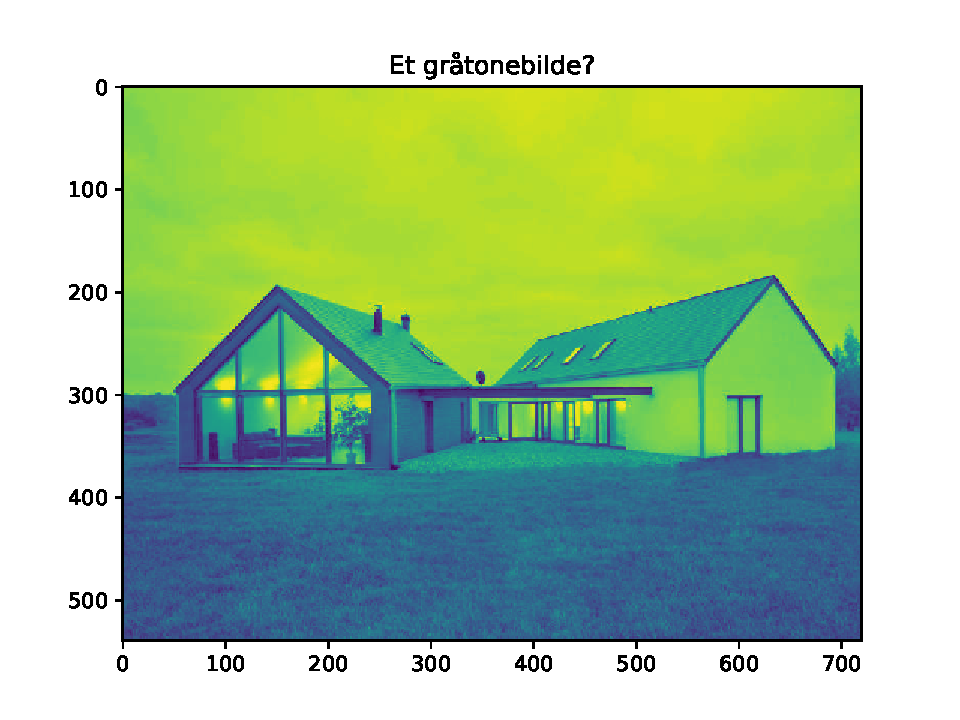
\includegraphics[width=0.9\linewidth]{Figure_1.pdf}}
  \caption{
  Bilde av det første vinduet.
  }
\end{figure}
%\clearpage % flush figures 



\begin{figure}[!ht]  % 
  \centerline{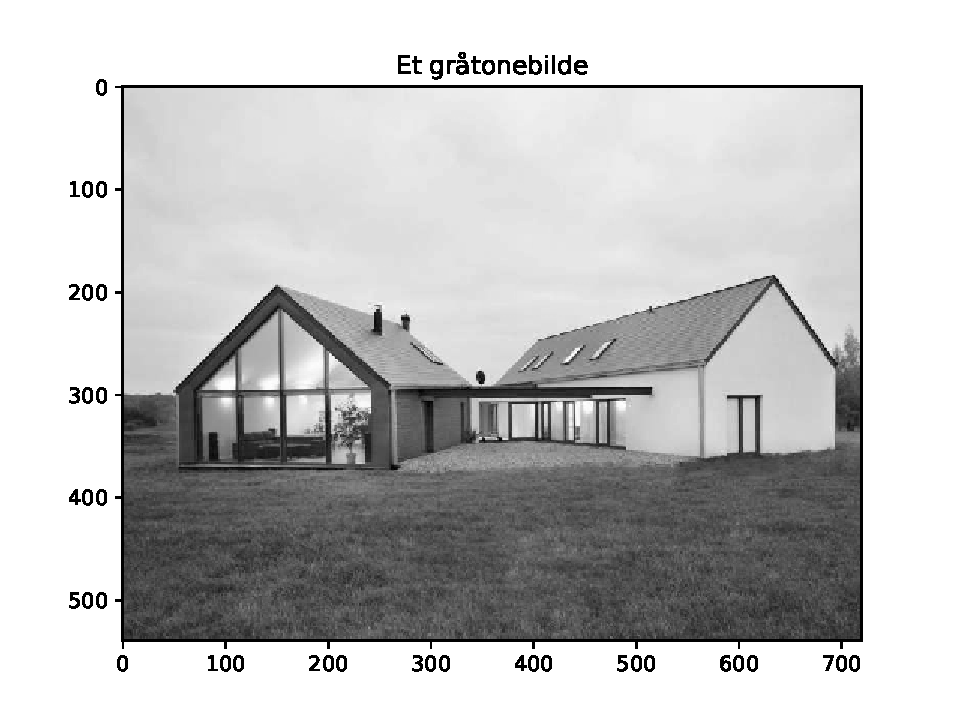
\includegraphics[width=0.9\linewidth]{Figure_2.pdf}}
  \caption{
  Bilde av det andre vinduet.
  }
\end{figure}
%\clearpage % flush figures 


Her kan du se at det første bilde ikke er gråtone - selvom det er tenkt et gråtonebilde. Dette skjer fordi \emph{matplotlib.pyplot} har en standard, predefinert måte å fremvise tallverdier som farger på.
Det må spesifiseres at en ønsker å framvise bildet som faktisk gråtone. Dette gjøres med å spesifisere et \emph{colormap} ved å sende inn som argument \emph{cmap=<ønsket colormap>}. Det finnes flere colormaps, hvis en ønsker å bruke det.

Dette er også viktig å bruke \textbf{figure()} hvis man ikke ønsker at det nye bildet som fremvises overlapper bildet som tidligere har blitt sendt inn til \emph{imshow}.



\vspace{3mm}


Det kan også hende at etter noen operasjoner at de matrisene en jobber med, har verdier som er større enn det et bilde bør ha. Et 8-bit bilde har verdier fra 0 til og med 255.
Ved fremvising, tilpasser matplotlib seg etter de verdiene som den innsendte matrisen har. Dette kan føre til at vi ikke ser resultatene etter å ha utført noen operasjoner.
For å sørge for at matplotlib viser bildet som om den har verdier mellom 0 og 255, må en bruke \emph{vmin} og \emph{vmax}:
\begin{minted}[fontsize=\fontsize{9pt}{9pt},linenos=false,mathescape,baselinestretch=1.0,fontfamily=tt,xleftmargin=2mm]{python}
plt.imshow(img,vmin=0,vmax=255)
\end{minted}



\vspace{3mm}


Noen ganger kan bildet se lite ut i vinduet. Det er mulig at matplotlib skalerer bildet slik at det fyller hele vinduet. Det gjøres slik:
\begin{minted}[fontsize=\fontsize{9pt}{9pt},linenos=false,mathescape,baselinestretch=1.0,fontfamily=tt,xleftmargin=2mm]{python}
plt.imshow(<bilde og andre argumenter>, aspect='auto')
\end{minted}
\paragraph{En liten demonstrasjon.}
\label{subsec:demo}
Denne demonstrasjonen oppsummerer det som har vært beskrevet i denne innledningen. Dette er kanskje en av de funksjonskallene som vil bli brukt i programmene, og som er ganske nyttige
for å se hvordan et bilde forandrer seg i løpet av et program.

Bildebehandling er et fag der eksperimentering er viktig, og da er det nyttig å vise fram og presentere resultatene programmet har fått.

\begin{minted}[fontsize=\fontsize{9pt}{9pt},linenos=false,mathescape,baselinestretch=1.0,fontfamily=tt,xleftmargin=2mm]{python}
from scipy.misc import imread
import matplotlib.pyplot as plt
import numpy as np

img = imread("houses.png",flatten=True)

plt.imshow(img,cmap='gray')
plt.title("Originalbilde")

# Øke kontrast
img_increased_contrast = img*1.5

# Gjøre bildet lysere
img_brighter = img + 100

plt.figure()

plt.subplot(2,1,1) # subplot deler et vindu i flere delplott.
plt.imshow(img_increased_contrast,cmap='gray',vmin=0,vmax=255,aspect='auto')
plt.title("Økt kontrast")

plt.subplot(2,1,2)
plt.imshow(img_brighter,cmap='gray',vmin=0,vmax=255,aspect='auto')
plt.title("Økt lyshet")

plt.show()
\end{minted}
Programmet kan lastes ned \href{{https://github.com/krisbhei/INF2310/raw/master/Programmering/Python/demo.py}}{her} (høyreklikk og trykk "lagre lenke som"/"save link as")

God programmering!


% ------------------- end of main content ---------------

% #ifdef PREAMBLE
\end{document}
% #endif

